\documentclass[11pt,compress,t,notes=noshow, xcolor=table]{beamer}

\usepackage[]{graphicx}
\usepackage[]{color}
% maxwidth is the original width if it is less than linewidth
% otherwise use linewidth (to make sure the graphics do not exceed the margin)
\makeatletter
\def\maxwidth{ %
  \ifdim\Gin@nat@width>\linewidth
    \linewidth
  \else
    \Gin@nat@width
  \fi
}
\makeatother

% ---------------------------------%
% latex-math dependencies, do not remove:
% - mathtools
% - bm
% - siunitx
% - dsfont
% - xspace
% ---------------------------------%

%--------------------------------------------------------%
%       Language, encoding, typography
%--------------------------------------------------------%

\usepackage[english]{babel}
\usepackage[utf8]{inputenc} % Enables inputting UTF-8 symbols
% Standard AMS suite
\usepackage{amsmath,amsfonts,amssymb}

% Font for double-stroke / blackboard letters for sets of numbers (N, R, ...)
% Distribution name is "doublestroke"
% According to https://mirror.physik.tu-berlin.de/pub/CTAN/fonts/doublestroke/dsdoc.pdf
% the "bbm" package does a similar thing and may be superfluous.
% Required for latex-math
\usepackage{dsfont}

% bbm – "Blackboard-style" cm fonts (https://www.ctan.org/pkg/bbm)
% Used to be in common.tex, loaded directly after this file
% Maybe superfluous given dsfont is loaded
% TODO: Check if really unused?
% \usepackage{bbm}

% bm – Access bold symbols in maths mode - https://ctan.org/pkg/bm
% Required for latex-math
% https://tex.stackexchange.com/questions/3238/bm-package-versus-boldsymbol
\usepackage{bm}

% pifont – Access to PostScript standard Symbol and Dingbats fonts
% Used for \newcommand{\xmark}{\ding{55}, which is never used
% aside from lecture_advml/attic/xx-automl/slides.Rnw
% \usepackage{pifont}

% Quotes (inline and display), provdes \enquote
% https://ctan.org/pkg/csquotes
\usepackage{csquotes}

% Adds arg to enumerate env, technically superseded by enumitem according
% to https://ctan.org/pkg/enumerate
% Replace with https://ctan.org/pkg/enumitem ?
\usepackage{enumerate}

% Line spacing - provides \singlespacing \doublespacing \onehalfspacing
% https://ctan.org/pkg/setspace
% \usepackage{setspace}

% mathtools – Mathematical tools to use with amsmath
% https://ctan.org/pkg/mathtools?lang=en
% latex-math dependency according to latex-math repo
\usepackage{mathtools}

% Maybe not great to use this https://tex.stackexchange.com/a/197/19093
% Use align instead -- TODO: Global search & replace to check, eqnarray is used a lot
% $ rg -f -u "\begin{eqnarray" -l | grep -v attic | awk -F '/' '{print $1}' | sort | uniq -c
%   13 lecture_advml
%   14 lecture_i2ml
%    2 lecture_iml
%   27 lecture_optimization
%   45 lecture_sl
\usepackage{eqnarray}

% For shaded regions / boxes
% Used sometimes in optim
% https://www.ctan.org/pkg/framed
\usepackage{framed}

%--------------------------------------------------------%
%       Cite button (version 2024-05)
%--------------------------------------------------------%
% Note this requires biber to be in $PATH when running,
% telltale error in log would be e.g. Package biblatex Info: ... file 'authoryear.dbx' not found
% aside from obvious "biber: command not found" or similar.

\usepackage{hyperref}
\usepackage{usebib}
\usepackage[backend=biber, style=authoryear]{biblatex}

% Only try adding a references file if it exists, otherwise
% this would compile error when references.bib is not found
\IfFileExists{references.bib} {
  \addbibresource{references.bib}
  \bibinput{references}
}

\newcommand{\citelink}[1]{%
\NoCaseChange{\resizebox{!}{9pt}{\protect\beamergotobutton{\href{\usebibentry{\NoCaseChange{#1}}{url}}{\begin{NoHyper}\cite{#1}\end{NoHyper}}}}}%
}

%--------------------------------------------------------%
%       Displaying code and algorithms
%--------------------------------------------------------%

% Reimplements verbatim environments: https://ctan.org/pkg/verbatim
% verbatim used sed at least once in
% supervised-classification/slides-classification-tasks.tex
\usepackage{verbatim}

% Both used together for algorithm typesetting, see also overleaf: https://www.overleaf.com/learn/latex/Algorithms
% algorithmic env is also used, but part of the bundle:
%   "algpseudocode is part of the algorithmicx bundle, it gives you an improved version of algorithmic besides providing some other features"
% According to https://tex.stackexchange.com/questions/229355/algorithm-algorithmic-algorithmicx-algorithm2e-algpseudocode-confused
\usepackage{algorithm}
\usepackage{algpseudocode}

%--------------------------------------------------------%
%       Tables
%--------------------------------------------------------%

% multi-row table cells: https://www.namsu.de/Extra/pakete/Multirow.html
% Provides \multirow
% Used e.g. in evaluation/slides-evaluation-measures-classification.tex
\usepackage{multirow}

% colortbl: https://ctan.org/pkg/colortbl
% "The package allows rows and columns to be coloured, and even individual cells." well.
% Provides \columncolor and \rowcolor
% \rowcolor is used multiple times, e.g. in knn/slides-knn.tex
\usepackage{colortbl}

% long/multi-page tables: https://texdoc.org/serve/longtable.pdf/0
% Not used in slides
% \usepackage{longtable}

% pretty table env: https://ctan.org/pkg/booktabs
% Is used
% Defines \toprule
\usepackage{booktabs}

%--------------------------------------------------------%
%       Figures: Creating, placing, verbing
%--------------------------------------------------------%

% wrapfig - Wrapping text around figures https://de.overleaf.com/learn/latex/Wrapping_text_around_figures
% Provides wrapfigure environment -used in lecture_optimization
\usepackage{wrapfig}

% Sub figures in figures and tables
% https://ctan.org/pkg/subfig -- supersedes subfigure package
% Provides \subfigure
% \subfigure not used in slides but slides-tuning-practical.pdf errors without this pkg, error due to \captionsetup undefined
\usepackage{subfig}

% Actually it's pronounced PGF https://en.wikibooks.org/wiki/LaTeX/PGF/TikZ
\usepackage{tikz}

% No idea what/why these settings are what they are but I assume they're there on purpose
\usetikzlibrary{shapes,arrows,automata,positioning,calc,chains,trees, shadows}
\tikzset{
  %Define standard arrow tip
  >=stealth',
  %Define style for boxes
  punkt/.style={
    rectangle,
    rounded corners,
    draw=black, very thick,
    text width=6.5em,
    minimum height=2em,
    text centered},
  % Define arrow style
  pil/.style={
    ->,
    thick,
    shorten <=2pt,
    shorten >=2pt,}
}

% Defines macros and environments
\usepackage{../../style/lmu-lecture}

\let\code=\texttt     % Used regularly

% Not sure what/why this does
\setkeys{Gin}{width=0.9\textwidth}

% -- knitr leftovers --
% Used often in conjunction with \definecolor{shadecolor}{rgb}{0.969, 0.969, 0.969}
% Removing definitions requires chaning _many many_ slides, which then need checking to see if output still ok
\definecolor{fgcolor}{rgb}{0.345, 0.345, 0.345}
\definecolor{shadecolor}{rgb}{0.969, 0.969, 0.969}
\newenvironment{knitrout}{}{} % an empty environment to be redefined in TeX

%-------------------------------------------------------------------------------------------------------%
%  Unused stuff that needs to go but is kept here currently juuuust in case it was important after all  %
%-------------------------------------------------------------------------------------------------------%

% \newcommand{\hlnum}[1]{\textcolor[rgb]{0.686,0.059,0.569}{#1}}%
% \newcommand{\hlstr}[1]{\textcolor[rgb]{0.192,0.494,0.8}{#1}}%
% \newcommand{\hlcom}[1]{\textcolor[rgb]{0.678,0.584,0.686}{\textit{#1}}}%
% \newcommand{\hlopt}[1]{\textcolor[rgb]{0,0,0}{#1}}%
% \newcommand{\hlstd}[1]{\textcolor[rgb]{0.345,0.345,0.345}{#1}}%
% \newcommand{\hlkwa}[1]{\textcolor[rgb]{0.161,0.373,0.58}{\textbf{#1}}}%
% \newcommand{\hlkwb}[1]{\textcolor[rgb]{0.69,0.353,0.396}{#1}}%
% \newcommand{\hlkwc}[1]{\textcolor[rgb]{0.333,0.667,0.333}{#1}}%
% \newcommand{\hlkwd}[1]{\textcolor[rgb]{0.737,0.353,0.396}{\textbf{#1}}}%
% \let\hlipl\hlkwb

% \makeatletter
% \newenvironment{kframe}{%
%  \def\at@end@of@kframe{}%
%  \ifinner\ifhmode%
%   \def\at@end@of@kframe{\end{minipage}}%
%   \begin{minipage}{\columnwidth}%
%  \fi\fi%
%  \def\FrameCommand##1{\hskip\@totalleftmargin \hskip-\fboxsep
%  \colorbox{shadecolor}{##1}\hskip-\fboxsep
%      % There is no \\@totalrightmargin, so:
%      \hskip-\linewidth \hskip-\@totalleftmargin \hskip\columnwidth}%
%  \MakeFramed {\advance\hsize-\width
%    \@totalleftmargin\z@ \linewidth\hsize
%    \@setminipage}}%
%  {\par\unskip\endMakeFramed%
%  \at@end@of@kframe}
% \makeatother

% \definecolor{shadecolor}{rgb}{.97, .97, .97}
% \definecolor{messagecolor}{rgb}{0, 0, 0}
% \definecolor{warningcolor}{rgb}{1, 0, 1}
% \definecolor{errorcolor}{rgb}{1, 0, 0}
% \newenvironment{knitrout}{}{} % an empty environment to be redefined in TeX

% \usepackage{alltt}
% \newcommand{\SweaveOpts}[1]{}  % do not interfere with LaTeX
% \newcommand{\SweaveInput}[1]{} % because they are not real TeX commands
% \newcommand{\Sexpr}[1]{}       % will only be parsed by R
% \newcommand{\xmark}{\ding{55}}%

% textpos – Place boxes at arbitrary positions on the LATEX page
% https://ctan.org/pkg/textpos
% Provides \begin{textblock}
% TODO: Check if really unused?
% \usepackage[absolute,overlay]{textpos}

% -----------------------%
% Likely knitr leftovers %
% -----------------------%

% psfrag – Replace strings in encapsulated PostScript figures
% https://www.overleaf.com/latex/examples/psfrag-example/tggxhgzwrzhn
% https://ftp.mpi-inf.mpg.de/pub/tex/mirror/ftp.dante.de/pub/tex/macros/latex/contrib/psfrag/pfgguide.pdf
% Can't tell if this is needed
% TODO: Check if really unused?
% \usepackage{psfrag}

% arydshln – Draw dash-lines in array/tabular
% https://www.ctan.org/pkg/arydshln
% !! "arydshln has to be loaded after array, longtable, colortab and/or colortbl"
% Provides \hdashline and \cdashline
% Not used in slides
% \usepackage{arydshln}

% tabularx – Tabulars with adjustable-width columns
% https://ctan.org/pkg/tabularx
% Provides \begin{tabularx}
% Not used in slides
% \usepackage{tabularx}

% placeins – Control float placement
% https://ctan.org/pkg/placeins
% Defines a \FloatBarrier command
% TODO: Check if really unused?
% \usepackage{placeins}

% Can't find a reason why common.tex is not just part of this file?
% This file is included in slides and exercises

% Rarely used fontstyle for R packages, used only in 
% - forests/slides-forests-benchmark.tex
% - exercises/single-exercises/methods_l_1.Rnw
% - slides/cart/attic/slides_extra_trees.Rnw
\newcommand{\pkg}[1]{{\fontseries{b}\selectfont #1}}

% Spacing helpers, used often (mostly in exercises for \dlz)
\newcommand{\lz}{\vspace{0.5cm}} % vertical space (used often in slides)
\newcommand{\dlz}{\vspace{1cm}}  % double vertical space (used often in exercises, never in slides)

% Don't know if this is used or needed, remove?
% textcolor that works in mathmode
% https://tex.stackexchange.com/a/261480
% Used e.g. in forests/slides-forests-bagging.tex
% [...] \textcolor{blue}{\tfrac{1}{M}\sum^M_{m} [...]
% \makeatletter
% \renewcommand*{\@textcolor}[3]{%
%   \protect\leavevmode
%   \begingroup
%     \color#1{#2}#3%
%   \endgroup
% }
% \makeatother


% dependencies: amsmath, amssymb, dsfont
% math spaces
\ifdefined\N
\renewcommand{\N}{\mathds{N}} % N, naturals
\else \newcommand{\N}{\mathds{N}} \fi
\newcommand{\Z}{\mathds{Z}} % Z, integers
\newcommand{\Q}{\mathds{Q}} % Q, rationals
\newcommand{\R}{\mathds{R}} % R, reals
\ifdefined\C
\renewcommand{\C}{\mathds{C}} % C, complex
\else \newcommand{\C}{\mathds{C}} \fi
\newcommand{\continuous}{\mathcal{C}} % C, space of continuous functions
\newcommand{\M}{\mathcal{M}} % machine numbers
\newcommand{\epsm}{\epsilon_m} % maximum error

% counting / finite sets
\newcommand{\setzo}{\{0, 1\}} % set 0, 1
\newcommand{\setmp}{\{-1, +1\}} % set -1, 1
\newcommand{\unitint}{[0, 1]} % unit interval

% basic math stuff
\newcommand{\xt}{\tilde x} % x tilde
\DeclareMathOperator*{\argmax}{arg\,max} % argmax
\DeclareMathOperator*{\argmin}{arg\,min} % argmin
\newcommand{\argminlim}{\mathop{\mathrm{arg\,min}}\limits} % argmax with limits
\newcommand{\argmaxlim}{\mathop{\mathrm{arg\,max}}\limits} % argmin with limits
\newcommand{\sign}{\operatorname{sign}} % sign, signum
\newcommand{\I}{\mathbb{I}} % I, indicator
\newcommand{\order}{\mathcal{O}} % O, order
\newcommand{\bigO}{\mathcal{O}} % Big-O Landau
\newcommand{\littleo}{{o}} % Little-o Landau
\newcommand{\pd}[2]{\frac{\partial{#1}}{\partial #2}} % partial derivative
\newcommand{\floorlr}[1]{\left\lfloor #1 \right\rfloor} % floor
\newcommand{\ceillr}[1]{\left\lceil #1 \right\rceil} % ceiling
\newcommand{\indep}{\perp \!\!\! \perp} % independence symbol

% sums and products
\newcommand{\sumin}{\sum\limits_{i=1}^n} % summation from i=1 to n
\newcommand{\sumim}{\sum\limits_{i=1}^m} % summation from i=1 to m
\newcommand{\sumjn}{\sum\limits_{j=1}^n} % summation from j=1 to p
\newcommand{\sumjp}{\sum\limits_{j=1}^p} % summation from j=1 to p
\newcommand{\sumik}{\sum\limits_{i=1}^k} % summation from i=1 to k
\newcommand{\sumkg}{\sum\limits_{k=1}^g} % summation from k=1 to g
\newcommand{\sumjg}{\sum\limits_{j=1}^g} % summation from j=1 to g
\newcommand{\summM}{\sum\limits_{m=1}^M} % summation from m=1 to M
\newcommand{\meanin}{\frac{1}{n} \sum\limits_{i=1}^n} % mean from i=1 to n
\newcommand{\meanim}{\frac{1}{m} \sum\limits_{i=1}^m} % mean from i=1 to n
\newcommand{\meankg}{\frac{1}{g} \sum\limits_{k=1}^g} % mean from k=1 to g
\newcommand{\meanmM}{\frac{1}{M} \sum\limits_{m=1}^M} % mean from m=1 to M
\newcommand{\prodin}{\prod\limits_{i=1}^n} % product from i=1 to n
\newcommand{\prodkg}{\prod\limits_{k=1}^g} % product from k=1 to g
\newcommand{\prodjp}{\prod\limits_{j=1}^p} % product from j=1 to p

% linear algebra
\newcommand{\one}{\bm{1}} % 1, unitvector
\newcommand{\zero}{\mathbf{0}} % 0-vector
\newcommand{\id}{\bm{I}} % I, identity
\newcommand{\diag}{\operatorname{diag}} % diag, diagonal
\newcommand{\trace}{\operatorname{tr}} % tr, trace
\newcommand{\spn}{\operatorname{span}} % span
\newcommand{\scp}[2]{\left\langle #1, #2 \right\rangle} % <.,.>, scalarproduct
\newcommand{\mat}[1]{\begin{pmatrix} #1 \end{pmatrix}} % short pmatrix command
\newcommand{\Amat}{\mathbf{A}} % matrix A
\newcommand{\Deltab}{\mathbf{\Delta}} % error term for vectors

% basic probability + stats
\renewcommand{\P}{\mathds{P}} % P, probability
\newcommand{\E}{\mathds{E}} % E, expectation
\newcommand{\var}{\mathsf{Var}} % Var, variance
\newcommand{\cov}{\mathsf{Cov}} % Cov, covariance
\newcommand{\corr}{\mathsf{Corr}} % Corr, correlation
\newcommand{\normal}{\mathcal{N}} % N of the normal distribution
\newcommand{\iid}{\overset{i.i.d}{\sim}} % dist with i.i.d superscript
\newcommand{\distas}[1]{\overset{#1}{\sim}} % ... is distributed as ...

% machine learning
\newcommand{\Xspace}{\mathcal{X}} % X, input space
\newcommand{\Yspace}{\mathcal{Y}} % Y, output space
\newcommand{\Zspace}{\mathcal{Z}} % Z, space of sampled datapoints
\newcommand{\nset}{\{1, \ldots, n\}} % set from 1 to n
\newcommand{\pset}{\{1, \ldots, p\}} % set from 1 to p
\newcommand{\gset}{\{1, \ldots, g\}} % set from 1 to g
\newcommand{\Pxy}{\mathbb{P}_{xy}} % P_xy
\newcommand{\Exy}{\mathbb{E}_{xy}} % E_xy: Expectation over random variables xy
\newcommand{\xv}{\mathbf{x}} % vector x (bold)
\newcommand{\xtil}{\tilde{\mathbf{x}}} % vector x-tilde (bold)
\newcommand{\yv}{\mathbf{y}} % vector y (bold)
\newcommand{\xy}{(\xv, y)} % observation (x, y)
\newcommand{\xvec}{\left(x_1, \ldots, x_p\right)^\top} % (x1, ..., xp)
\newcommand{\Xmat}{\mathbf{X}} % Design matrix
\newcommand{\allDatasets}{\mathds{D}} % The set of all datasets
\newcommand{\allDatasetsn}{\mathds{D}_n}  % The set of all datasets of size n
\newcommand{\D}{\mathcal{D}} % D, data
\newcommand{\Dn}{\D_n} % D_n, data of size n
\newcommand{\Dtrain}{\mathcal{D}_{\text{train}}} % D_train, training set
\newcommand{\Dtest}{\mathcal{D}_{\text{test}}} % D_test, test set
\newcommand{\xyi}[1][i]{\left(\xv^{(#1)}, y^{(#1)}\right)} % (x^i, y^i), i-th observation
\newcommand{\Dset}{\left( \xyi[1], \ldots, \xyi[n]\right)} % {(x1,y1)), ..., (xn,yn)}, data
\newcommand{\defAllDatasetsn}{(\Xspace \times \Yspace)^n} % Def. of the set of all datasets of size n
\newcommand{\defAllDatasets}{\bigcup_{n \in \N}(\Xspace \times \Yspace)^n} % Def. of the set of all datasets
\newcommand{\xdat}{\left\{ \xv^{(1)}, \ldots, \xv^{(n)}\right\}} % {x1, ..., xn}, input data
\newcommand{\ydat}{\left\{ \yv^{(1)}, \ldots, \yv^{(n)}\right\}} % {y1, ..., yn}, input data
\newcommand{\yvec}{\left(y^{(1)}, \hdots, y^{(n)}\right)^\top} % (y1, ..., yn), vector of outcomes
\newcommand{\greekxi}{\xi} % Greek letter xi
\renewcommand{\xi}[1][i]{\xv^{(#1)}} % x^i, i-th observed value of x
\newcommand{\yi}[1][i]{y^{(#1)}} % y^i, i-th observed value of y
\newcommand{\xivec}{\left(x^{(i)}_1, \ldots, x^{(i)}_p\right)^\top} % (x1^i, ..., xp^i), i-th observation vector
\newcommand{\xj}{\xv_j} % x_j, j-th feature
\newcommand{\xjvec}{\left(x^{(1)}_j, \ldots, x^{(n)}_j\right)^\top} % (x^1_j, ..., x^n_j), j-th feature vector
\newcommand{\phiv}{\mathbf{\phi}} % Basis transformation function phi
\newcommand{\phixi}{\mathbf{\phi}^{(i)}} % Basis transformation of xi: phi^i := phi(xi)

%%%%%% ml - models general
\newcommand{\lamv}{\bm{\lambda}} % lambda vector, hyperconfiguration vector
\newcommand{\Lam}{\bm{\Lambda}}	 % Lambda, space of all hpos
% Inducer / Inducing algorithm
\newcommand{\preimageInducer}{\left(\defAllDatasets\right)\times\Lam} % Set of all datasets times the hyperparameter space
\newcommand{\preimageInducerShort}{\allDatasets\times\Lam} % Set of all datasets times the hyperparameter space
% Inducer / Inducing algorithm
\newcommand{\ind}{\mathcal{I}} % Inducer, inducing algorithm, learning algorithm

% continuous prediction function f
\newcommand{\ftrue}{f_{\text{true}}}  % True underlying function (if a statistical model is assumed)
\newcommand{\ftruex}{\ftrue(\xv)} % True underlying function (if a statistical model is assumed)
\newcommand{\fx}{f(\xv)} % f(x), continuous prediction function
\newcommand{\fdomains}{f: \Xspace \rightarrow \R^g} % f with domain and co-domain
\newcommand{\Hspace}{\mathcal{H}} % hypothesis space where f is from
\newcommand{\fbayes}{f^{\ast}} % Bayes-optimal model
\newcommand{\fxbayes}{f^{\ast}(\xv)} % Bayes-optimal model
\newcommand{\fkx}[1][k]{f_{#1}(\xv)} % f_j(x), discriminant component function
\newcommand{\fh}{\hat{f}} % f hat, estimated prediction function
\newcommand{\fxh}{\fh(\xv)} % fhat(x)
\newcommand{\fxt}{f(\xv ~|~ \thetav)} % f(x | theta)
\newcommand{\fxi}{f\left(\xv^{(i)}\right)} % f(x^(i))
\newcommand{\fxih}{\hat{f}\left(\xv^{(i)}\right)} % f(x^(i))
\newcommand{\fxit}{f\left(\xv^{(i)} ~|~ \thetav\right)} % f(x^(i) | theta)
\newcommand{\fhD}{\fh_{\D}} % fhat_D, estimate of f based on D
\newcommand{\fhDtrain}{\fh_{\Dtrain}} % fhat_Dtrain, estimate of f based on D
\newcommand{\fhDnlam}{\fh_{\Dn, \lamv}} %model learned on Dn with hp lambda
\newcommand{\fhDlam}{\fh_{\D, \lamv}} %model learned on D with hp lambda
\newcommand{\fhDnlams}{\fh_{\Dn, \lamv^\ast}} %model learned on Dn with optimal hp lambda
\newcommand{\fhDlams}{\fh_{\D, \lamv^\ast}} %model learned on D with optimal hp lambda

% discrete prediction function h
\newcommand{\hx}{h(\xv)} % h(x), discrete prediction function
\newcommand{\hh}{\hat{h}} % h hat
\newcommand{\hxh}{\hat{h}(\xv)} % hhat(x)
\newcommand{\hxt}{h(\xv | \thetav)} % h(x | theta)
\newcommand{\hxi}{h\left(\xi\right)} % h(x^(i))
\newcommand{\hxit}{h\left(\xi ~|~ \thetav\right)} % h(x^(i) | theta)
\newcommand{\hbayes}{h^{\ast}} % Bayes-optimal classification model
\newcommand{\hxbayes}{h^{\ast}(\xv)} % Bayes-optimal classification model

% yhat
\newcommand{\yh}{\hat{y}} % yhat for prediction of target
\newcommand{\yih}{\hat{y}^{(i)}} % yhat^(i) for prediction of ith targiet
\newcommand{\resi}{\yi- \yih}

% theta
\newcommand{\thetah}{\hat{\theta}} % theta hat
\newcommand{\thetav}{\bm{\theta}} % theta vector
\newcommand{\thetavh}{\bm{\hat\theta}} % theta vector hat
\newcommand{\thetat}[1][t]{\thetav^{[#1]}} % theta^[t] in optimization
\newcommand{\thetatn}[1][t]{\thetav^{[#1 +1]}} % theta^[t+1] in optimization
\newcommand{\thetahDnlam}{\thetavh_{\Dn, \lamv}} %theta learned on Dn with hp lambda
\newcommand{\thetahDlam}{\thetavh_{\D, \lamv}} %theta learned on D with hp lambda
\newcommand{\mint}{\min_{\thetav \in \Theta}} % min problem theta
\newcommand{\argmint}{\argmin_{\thetav \in \Theta}} % argmin theta
% LS 29.10.2024 addin thetab back for now because apparently this broke and nobody updated slides to reflect thetab -> thetav changes?
\newcommand{\thetab}{\bm{\theta}} % theta vector


% densities + probabilities
% pdf of x
\newcommand{\pdf}{p} % p
\newcommand{\pdfx}{p(\xv)} % p(x)
\newcommand{\pixt}{\pi(\xv~|~ \thetav)} % pi(x|theta), pdf of x given theta
\newcommand{\pixit}[1][i]{\pi\left(\xi[#1] ~|~ \thetav\right)} % pi(x^i|theta), pdf of x given theta
\newcommand{\pixii}[1][i]{\pi\left(\xi[#1]\right)} % pi(x^i), pdf of i-th x

% pdf of (x, y)
\newcommand{\pdfxy}{p(\xv,y)} % p(x, y)
\newcommand{\pdfxyt}{p(\xv, y ~|~ \thetav)} % p(x, y | theta)
\newcommand{\pdfxyit}{p\left(\xi, \yi ~|~ \thetav\right)} % p(x^(i), y^(i) | theta)

% pdf of x given y
\newcommand{\pdfxyk}[1][k]{p(\xv | y= #1)} % p(x | y = k)
\newcommand{\lpdfxyk}[1][k]{\log p(\xv | y= #1)} % log p(x | y = k)
\newcommand{\pdfxiyk}[1][k]{p\left(\xi | y= #1 \right)} % p(x^i | y = k)

% prior probabilities
\newcommand{\pik}[1][k]{\pi_{#1}} % pi_k, prior
\newcommand{\lpik}[1][k]{\log \pi_{#1}} % log pi_k, log of the prior
\newcommand{\pit}{\pi(\thetav)} % Prior probability of parameter theta

% posterior probabilities
\newcommand{\post}{\P(y = 1 ~|~ \xv)} % P(y = 1 | x), post. prob for y=1
\newcommand{\postk}[1][k]{\P(y = #1 ~|~ \xv)} % P(y = k | y), post. prob for y=k
\newcommand{\pidomains}{\pi: \Xspace \rightarrow \unitint} % pi with domain and co-domain
\newcommand{\pibayes}{\pi^{\ast}} % Bayes-optimal classification model
\newcommand{\pixbayes}{\pi^{\ast}(\xv)} % Bayes-optimal classification model
\newcommand{\pix}{\pi(\xv)} % pi(x), P(y = 1 | x)
\newcommand{\piv}{\bm{\pi}} % pi, bold, as vector
\newcommand{\pikx}[1][k]{\pi_{#1}(\xv)} % pi_k(x), P(y = k | x)
\newcommand{\pikxt}[1][k]{\pi_{#1}(\xv ~|~ \thetav)} % pi_k(x | theta), P(y = k | x, theta)
\newcommand{\pixh}{\hat \pi(\xv)} % pi(x) hat, P(y = 1 | x) hat
\newcommand{\pikxh}[1][k]{\hat \pi_{#1}(\xv)} % pi_k(x) hat, P(y = k | x) hat
\newcommand{\pixih}{\hat \pi(\xi)} % pi(x^(i)) with hat
\newcommand{\pikxih}[1][k]{\hat \pi_{#1}(\xi)} % pi_k(x^(i)) with hat
\newcommand{\pdfygxt}{p(y ~|~\xv, \thetav)} % p(y | x, theta)
\newcommand{\pdfyigxit}{p\left(\yi ~|~\xi, \thetav\right)} % p(y^i |x^i, theta)
\newcommand{\lpdfygxt}{\log \pdfygxt } % log p(y | x, theta)
\newcommand{\lpdfyigxit}{\log \pdfyigxit} % log p(y^i |x^i, theta)

% probababilistic
\newcommand{\bayesrulek}[1][k]{\frac{\P(\xv | y= #1) \P(y= #1)}{\P(\xv)}} % Bayes rule
\newcommand{\muk}{\bm{\mu_k}} % mean vector of class-k Gaussian (discr analysis)

% residual and margin
\newcommand{\eps}{\epsilon} % residual, stochastic
\newcommand{\epsv}{\bm{\epsilon}} % residual, stochastic, as vector
\newcommand{\epsi}{\epsilon^{(i)}} % epsilon^i, residual, stochastic
\newcommand{\epsh}{\hat{\epsilon}} % residual, estimated
\newcommand{\epsvh}{\hat{\epsv}} % residual, estimated, vector
\newcommand{\yf}{y \fx} % y f(x), margin
\newcommand{\yfi}{\yi \fxi} % y^i f(x^i), margin
\newcommand{\Sigmah}{\hat \Sigma} % estimated covariance matrix
\newcommand{\Sigmahj}{\hat \Sigma_j} % estimated covariance matrix for the j-th class

% ml - loss, risk, likelihood
\newcommand{\Lyf}{L\left(y, f\right)} % L(y, f), loss function
\newcommand{\Lypi}{L\left(y, \pi\right)} % L(y, pi), loss function
\newcommand{\Lxy}{L\left(y, \fx\right)} % L(y, f(x)), loss function
\newcommand{\Lxyi}{L\left(\yi, \fxi\right)} % loss of observation
\newcommand{\Lxyt}{L\left(y, \fxt\right)} % loss with f parameterized
\newcommand{\Lxyit}{L\left(\yi, \fxit\right)} % loss of observation with f parameterized
\newcommand{\Lxym}{L\left(\yi, f\left(\bm{\tilde{x}}^{(i)} ~|~ \thetav\right)\right)} % loss of observation with f parameterized
\newcommand{\Lpixy}{L\left(y, \pix\right)} % loss in classification
\newcommand{\Lpiy}{L\left(y, \pi\right)} % loss in classification
\newcommand{\Lpiv}{L\left(y, \piv\right)} % loss in classification
\newcommand{\Lpixyi}{L\left(\yi, \pixii\right)} % loss of observation in classification
\newcommand{\Lpixyt}{L\left(y, \pixt\right)} % loss with pi parameterized
\newcommand{\Lpixyit}{L\left(\yi, \pixit\right)} % loss of observation with pi parameterized
\newcommand{\Lhy}{L\left(y, h\right)} % L(y, h), loss function on discrete classes
\newcommand{\Lhxy}{L\left(y, \hx\right)} % L(y, h(x)), loss function on discrete classes
\newcommand{\Lr}{L\left(r\right)} % L(r), loss defined on residual (reg) / margin (classif)
\newcommand{\lone}{|y - \fx|} % L1 loss
\newcommand{\ltwo}{\left(y - \fx\right)^2} % L2 loss
\newcommand{\lbernoullimp}{\ln(1 + \exp(-y \cdot \fx))} % Bernoulli loss for -1, +1 encoding
\newcommand{\lbernoullizo}{- y \cdot \fx + \log(1 + \exp(\fx))} % Bernoulli loss for 0, 1 encoding
\newcommand{\lcrossent}{- y \log \left(\pix\right) - (1 - y) \log \left(1 - \pix\right)} % cross-entropy loss
\newcommand{\lbrier}{\left(\pix - y \right)^2} % Brier score
\newcommand{\risk}{\mathcal{R}} % R, risk
\newcommand{\riskbayes}{\mathcal{R}^\ast}
\newcommand{\riskf}{\risk(f)} % R(f), risk
\newcommand{\riskdef}{\E_{y|\xv}\left(\Lxy \right)} % risk def (expected loss)
\newcommand{\riskt}{\mathcal{R}(\thetav)} % R(theta), risk
\newcommand{\riske}{\mathcal{R}_{\text{emp}}} % R_emp, empirical risk w/o factor 1 / n
\newcommand{\riskeb}{\bar{\mathcal{R}}_{\text{emp}}} % R_emp, empirical risk w/ factor 1 / n
\newcommand{\riskef}{\riske(f)} % R_emp(f)
\newcommand{\risket}{\mathcal{R}_{\text{emp}}(\thetav)} % R_emp(theta)
\newcommand{\riskr}{\mathcal{R}_{\text{reg}}} % R_reg, regularized risk
\newcommand{\riskrt}{\mathcal{R}_{\text{reg}}(\thetav)} % R_reg(theta)
\newcommand{\riskrf}{\riskr(f)} % R_reg(f)
\newcommand{\riskrth}{\hat{\mathcal{R}}_{\text{reg}}(\thetav)} % hat R_reg(theta)
\newcommand{\risketh}{\hat{\mathcal{R}}_{\text{emp}}(\thetav)} % hat R_emp(theta)
\newcommand{\LL}{\mathcal{L}} % L, likelihood
\newcommand{\LLt}{\mathcal{L}(\thetav)} % L(theta), likelihood
\newcommand{\LLtx}{\mathcal{L}(\thetav | \xv)} % L(theta|x), likelihood
\newcommand{\logl}{\ell} % l, log-likelihood
\newcommand{\loglt}{\logl(\thetav)} % l(theta), log-likelihood
\newcommand{\logltx}{\logl(\thetav | \xv)} % l(theta|x), log-likelihood
\newcommand{\errtrain}{\text{err}_{\text{train}}} % training error
\newcommand{\errtest}{\text{err}_{\text{test}}} % test error
\newcommand{\errexp}{\overline{\text{err}_{\text{test}}}} % avg training error

% lm
\newcommand{\thx}{\thetav^\top \xv} % linear model
\newcommand{\olsest}{(\Xmat^\top \Xmat)^{-1} \Xmat^\top \yv} % OLS estimator in LM



\newcommand{\titlefigure}{figure_man/NSGA2_CS2.png}
\newcommand{\learninggoals}{
\item A-Posteriori and EA
\item NSGA-II
\item SMS-EMOA algorithm
}


%\usepackage{animate} % only use if you want the animation for Taylor2D

\title{Optimization in Machine Learning}
%\author{Bernd Bischl}
\date{}

\begin{document}

\lecturechapter{Evolutionary multi-objective optimization algorithms (EMOA)}
\lecture{Optimization in Machine Learning}
\sloppy

%%%%%%%%%%%%%%%%%%%%%%%%%%%%%%%%%%%%%%%%%%%%%%%%%%%%%%%%%%%%%%%%%%%%%%%%%%%%%%%%%%%

%\begin{vbframe}{Notation}

%\begin{itemize}
%\item Admissible set $\Xspace \subset \R^n$
%\item Target region $\R^m$
%\item Multi-criteria objective function $f: \Xspace \to \R^m$
%\item Objective function vector $f(\bm{x}) = \left(f_1(\bm{x}), ..., f_m(\bm{x}\right))^\top \in \R^m$, which maps $\bm{x}$ into the space $\R^m$.
% \item $F:=f(\Xspace) = \left\{f(\bm{x}) ~|~ \bm{x} \in \Xspace\right\}$: Bild einer Funktion (Menge aller möglichen Funktionswerte)
%\end{itemize}

%w.l.o.g. we look at minimization problems.

%\end{vbframe}


% \begin{vbframe}{Skalarisierung}
%
% \textbf{Idee:} Führe mehrkriterielle Optimierung auf monokriterielle Optimierungsprobleme zurück.
%
% \lz
%
% Mögliches Verfahren: Optimiere eine gewichtete Summe
%
% $$
% w_1 \cdot f_1(\bm{x}) + w_2 \cdot f_2(\bm{x}) + ... + w_m \cdot f_m(\bm{x}),
% $$
%
% wobei $w_i \ge 0$ und $\sum_{i = 1}^m w_i = 1$ (Konvexkombination).
%
% \framebreak
%
% \textbf{Beispiel:} Es sei weiterhin $f_1(x) = (x - 1)^2$ und $f_2(x) = 3(x - 2)^2$. Wir lösen das skalare Ersatzproblem
%
% $$
% z = w_1 f_1(x) + w_2 f_2(x) = w_1 y_1 + w_2y_2 \to \min!
% $$
%
% Umformen ergibt hier eine Geradengleichung: $y_2 = -\frac{w_1}{w_2}y_1 + z$.
%
% \lz
%
% Grafisch finden wir das Optimum dieses skalaren Optimierungsproblems, indem wir
%
% \begin{itemize}
% \item alle möglichen Geraden $y_2 = -\frac{w_1}{w_2}y_1 + z$ für unterschiedliche Werte von $z$ einzeichnen und
% \item den Punkt finden, in dem sich die Gerade mit dem Bild der Funktion $F = f(\Xspace)$ berührt.
% \end{itemize}
%
% Beispielhaft für $w_2 = \frac{2}{3}$ und $w_1 = \frac{1}{3}$.
%
%<<echo = FALSE, fig.width = 2, fig.height=2, fig.align='center', warning=FALSE, include = FALSE>>=
%x = seq(-1, 4, length.out = 1000)
%lin = 3 * 0.4 - 2 * x
%fun1 = function(x) (x - 1)^2
%fun2 = function(x) 3 * (x - 2)^2
%
%p2 = ggplot() + geom_point(data = data.frame(f1 = fun1(x), f2 = fun2(x)), aes(x = f1, y = f2), size = 0.7)
%p2 = p2 + geom_line(aes(x = x, y = lin)) + ylim(c(-3, 25))
%p2 = p2 + geom_point(aes(x = 0.36, y = 0.48), colour = "green", size = 3)
%p2 = p2 + theme_bw()
%p2
%@

% \end{vbframe}
%
% \begin{vbframe}{Zusammenfassung: Skalarisierungsmethoden}
%
% Es gibt weitere Möglichkeiten, ein mehrkriterielles Problem durch eines oder mehrere skalare Ersatzprobleme approximativ zu löse (z.B. auch lexikografische Methode).
%
% \lz
%
% \textbf{Aber: }
%
% \begin{itemize}
% \item Aber: Es gibt Lösungen, die diesen Methoden verborgen bleiben (insbesondere: bei einmaliger Anwendung nur eine Lösunge)
% \item Auch monokriterielle Optimierung ist nicht immer \enquote{einfach}
% \end{itemize}
%
% \end{vbframe}
%
% \begin{vbframe}{Mehrkriterielles Abstiegsverfahren}
%
% Die Definition einer Abstiegsrichtung lässt sich auf den multikriteriellen Fall erweitern.
%
% \lz
%
% \textbf{Definition: } Abstiegsrichtung \\
% Es sei $f: \R^n \to \R^m$ stetig differenzierbar.  Eine Richtung $\bm{v} \in \R^n$ heißt \textbf{Abstiegsrichtung} in $\bm{x} \in \R^n$, wenn
%
% $$
% \nabla f_j(\bm{x})^T\bm{v} < 0 \quad \forall ~ j = 1, ..., m.
% $$
%
% \framebreak
%
% Problem: Das Finden einer Abstiegsrichtung ist per se schon ein nicht ganz einfach zu lösendes Problem.

%<<include = FALSE>>=
%f1 = function(x) 0.01 * sum(x^2) - 2
%f2 = function(x) 0.01 * sum(c(0.1, 0.3) * (x - c(-10, 20))^2)
%
%x1 = x2 = seq(-10, 20, length.out = 100)
%grid = expand.grid(x1 = x1, x2 = x2)
%grid$y1 = apply(grid[, 1:2], 1, f1)
%grid$y2 = apply(grid[, 1:2], 1, f2)
%
%melt = reshape2::melt(grid, id.vars = c("x1", "x2"))
%
%p = ggplot(data = melt) + geom_raster(aes(x = x1, y = x2, fill = value))
%p = p + geom_contour(aes(x = x1, y = x2, z = value, colour = variable), bins = 15)
%p = p + ylim(c(-20, 40)) + xlim(c(-20, 40)) + theme_bw()
%p
%@



%\section{Evolutionary multi-objective optimization algorithms (EMOA)}


\begin{vbframe}{A-posteriori methods and EA}

Evolutionary multi-objective algorithms (EMOAs) evolve a diverse population over time to approximate the Pareto front.

\begin{columns}
\begin{column}{0.3\textwidth}
\begin{center}
\begin{figure}
\centering
\begin{tikzpicture}[node distance=-1.8cm, auto,]
%nodes
\begin{footnotesize}
\node (init) {Initialize population};
\node[below = 0.1cm of init](rating1) {Eval population};
\node[below = 0.1cm of rating1](selection1) {Parent selection};
\node[below = 0.1cm of selection1](variation) {Variation};
\node[below = 0.1cm of variation](rating2) {Eval offspring};
\node[below = 0.1cm of rating2](selection2) {Survival selection};
\node[below = 0.1cm of selection2](stop) {Stop};
\node[below = 0.2cm of stop](dummy2) {};
\node[below = 0.2cm of stop](dummy3) {};
\node[right = 0.01cm of dummy3](dummy4) {yes};
\node[left = 0.2cm of rating2](dummy1) {no};
\draw[->] (init) to (rating1) node[midway, above]{};
\draw[->] (rating1) to (selection1) node[midway, above]{};
\draw[->] (selection1) to (variation) node[midway, above]{};
\draw[->] (variation) to (rating2) node[midway, above]{};
\draw[->] (rating2) to (selection2) node[midway, above]{};
\draw[->] (selection2) to (stop) node[midway, above]{};
\draw[->] (stop) to (dummy2) node[midway, above]{};
\draw[->] (stop) to [bend left=90, looseness=2](selection1) node[midway, above]{};
\end{footnotesize}
\end{tikzpicture}
\end{figure}
\end{center}
\begin{footnotesize}
\end{footnotesize}
\end{column}

  
\begin{column}{0.7\textwidth}
\vspace{0.6cm}  
\begin{center}
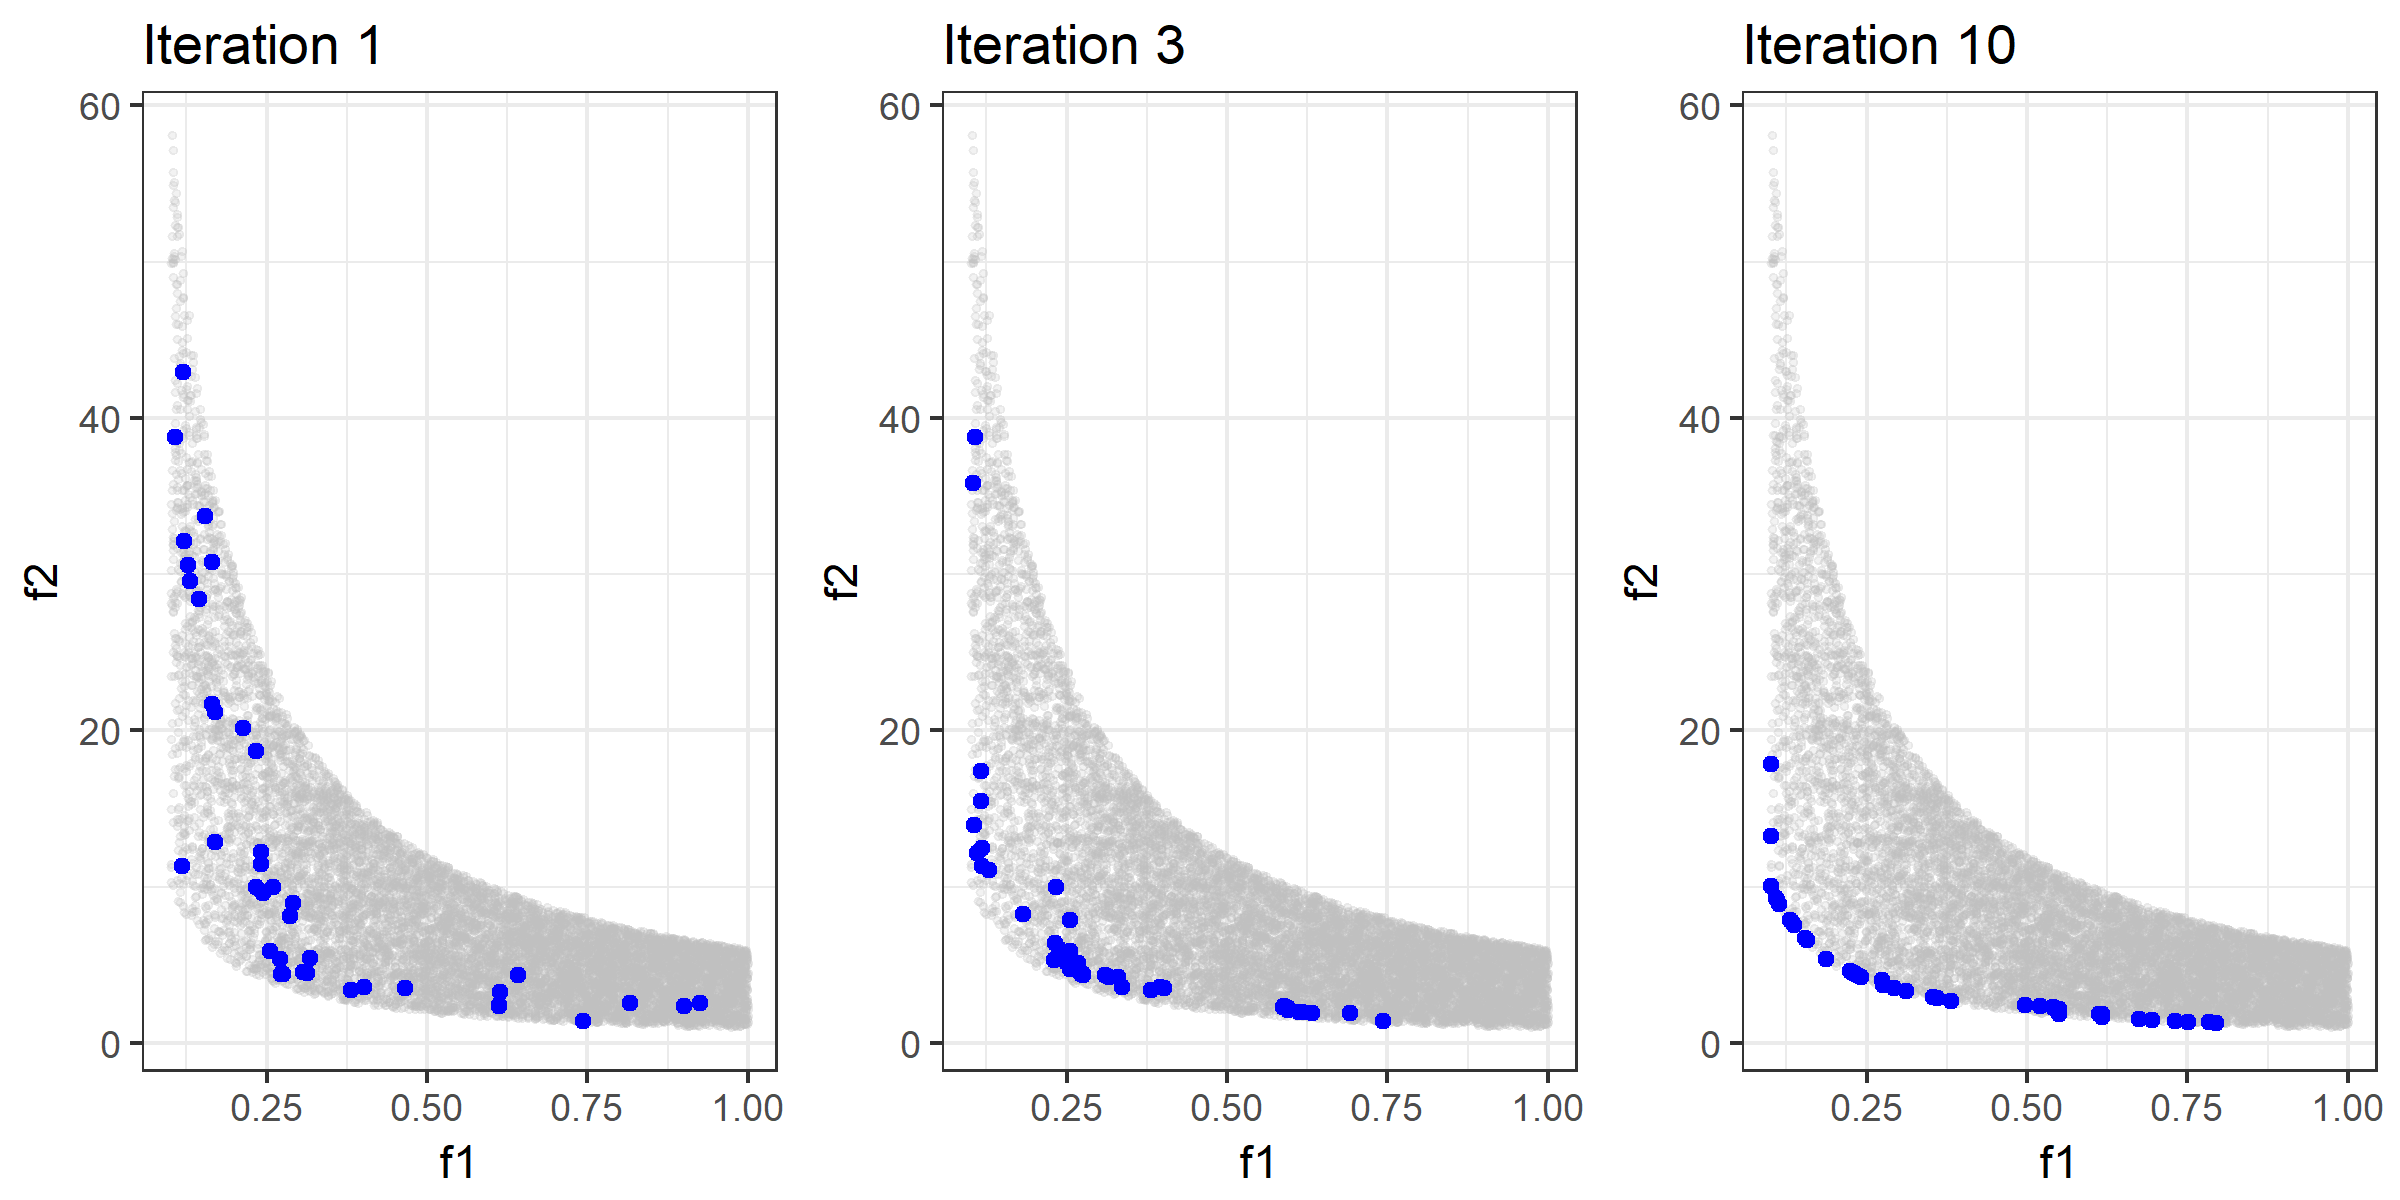
\includegraphics[width = 0.9\linewidth]{figure_man/EA-steps.png}
\end{center}
\end{column}
\end{columns}

\framebreak

%\begin{algorithm}[H]
 % \begin{center}
  %\caption{Basic EA template loop}
   %   \begin{algorithmic}[1]
    %      \STATE Init and eval population $\mathcal{P}_0 \subset \XX$ with $|\mathcal{P}| = \mu$ 
     % \STATE $t \leftarrow 0$
      %\REPEAT
       % \STATE Select parents and generate offspring $\mathcal{Q}_t$ with $|\mathcal{Q}_t| = \lambda$
        %\STATE Select $\mu$ survivors $\mathcal{P}_{t + 1}$ 
 	%	\STATE $t \leftarrow t + 1$
   %   \UNTIL{Stop criterion fulfilled}
    % \end{algorithmic}
    %\end{center}
%\end{algorithm}


\begin{algorithm}[H]
  \begin{center}
  \caption{Basic EA template loop}
    \begin{algorithmic}[1]
    \State Init and eval population $P_0 \subset \Xspace$ with $|P| = \mu$
    \State $t \leftarrow 0$
      \Repeat
        \State Select parents and generate offspring $Q_t$ with $|Q_t| = \lambda$
        \State Select $\mu$ survivors $P^{[t + 1]}$
        %\State Selection: select survivors $P_{t + 1}$
 		\State $t \leftarrow t + 1$
      \Until{Stop criterion fulfilled}
            \vspace*{-0.3cm}
    \end{algorithmic}
    \end{center}
\end{algorithm}

\begin{itemize}
   % \item Note that (as in the EA lecture unit) we are using somewhat non-standard notation here.
    \item Nearly all steps in the above template work also for EMOAs, but both parent and survival selection are now less obvious. How do we rank under multiple objectives?
\end{itemize}

%The population of solution candidates consists of $\bm{x} \in \Xspace$.

\end{vbframe}


%\begin{vbframe}{Objectives of an evolutionary strategy}

%The aim is to select the evolution strategy in such a way that the algorithm provides an approximation of the Pareto front, where

%\begin{enumerate}
%\item The individuals of the population (or the corresponding functional values in the target function space) \textbf{converge} to the Pareto front.
%\item The individuals of the population provide a \textbf{diverse} as possible approximation of the Pareto front.
%\end{enumerate}

%\vspace*{-0.3cm}

%\begin{center}
%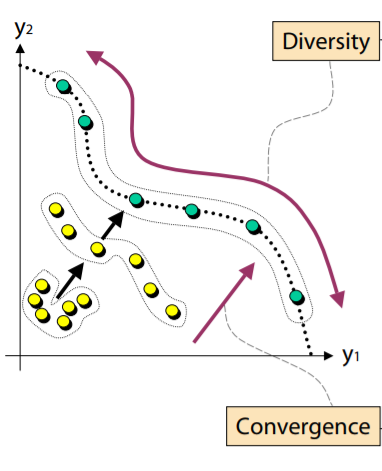
\includegraphics[width = 0.25\linewidth]{figure_man/EMO_goals.png}
%\end{center}

%\vspace*{-0.5cm}

%\begin{footnotesize}
%\textbf{Caution}: in this graphic the objective function values are exceptionally \textbf{maximized}.
%\end{footnotesize}

%\end{vbframe}

\begin{vbframe}{NSGA-II}

The \textbf{non-dominated sorting genetic algorithm (NSGA-II)} was published by {\href{https://www.iitk.ac.in/kangal/Deb_NSGA-II.pdf}{K. Dep et al. 2002}}.

\begin{itemize}
\item Follows a $(\mu + \lambda)$ strategy.
\item All previously discussed variation strategies can be used; 
    the original paper uses tournament selection, polynomial mutation and simulated binary crossover.
\item Parent and survival selection rank candidates by 
\begin{enumerate}
\item \textbf{Non-dominated sorting} as main criterion
\item \textbf{Crowding distance assignment} as tie breaker
\end{enumerate}
\end{itemize}

\end{vbframe}

\begin{vbframe}{NSGA-II: non-dominated sorting}

% \begin{center}
% 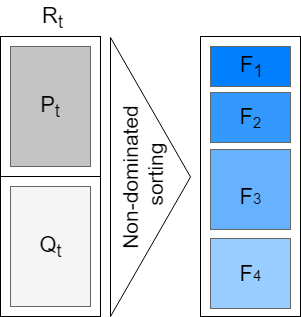
\includegraphics[width = 0.5\linewidth]{figure_man/NSGA2_1.png}
% \end{center}

% \framebreak

\begin{footnotesize}
NDS partitions an objective space set into fronts $\mathcal{F}_1 \prec \mathcal{F}_2 \prec \mathcal{F}_3 \prec ... $.

\begin{itemize}
    \item $\mathcal{F}_1$ is non-dominated, 
      each $\bm{x} \in \mathcal{F}_2$ is dominated, but only by points in $\mathcal{F}_1$, 
      each $\bm{x} \in \mathcal{F}_3$ is dominated, but only by points in $\mathcal{F}_1$ and $\mathcal{F}_2$, 
      and so on. 
    \item We can easily compute the partitioning by computing all non-dominated points  $\mathcal{F}_1$,
        removing them, then computing the next layer of non-dominated points $\mathcal{F}_2$, and so on.
\end{itemize}
\end{footnotesize}

\begin{center}
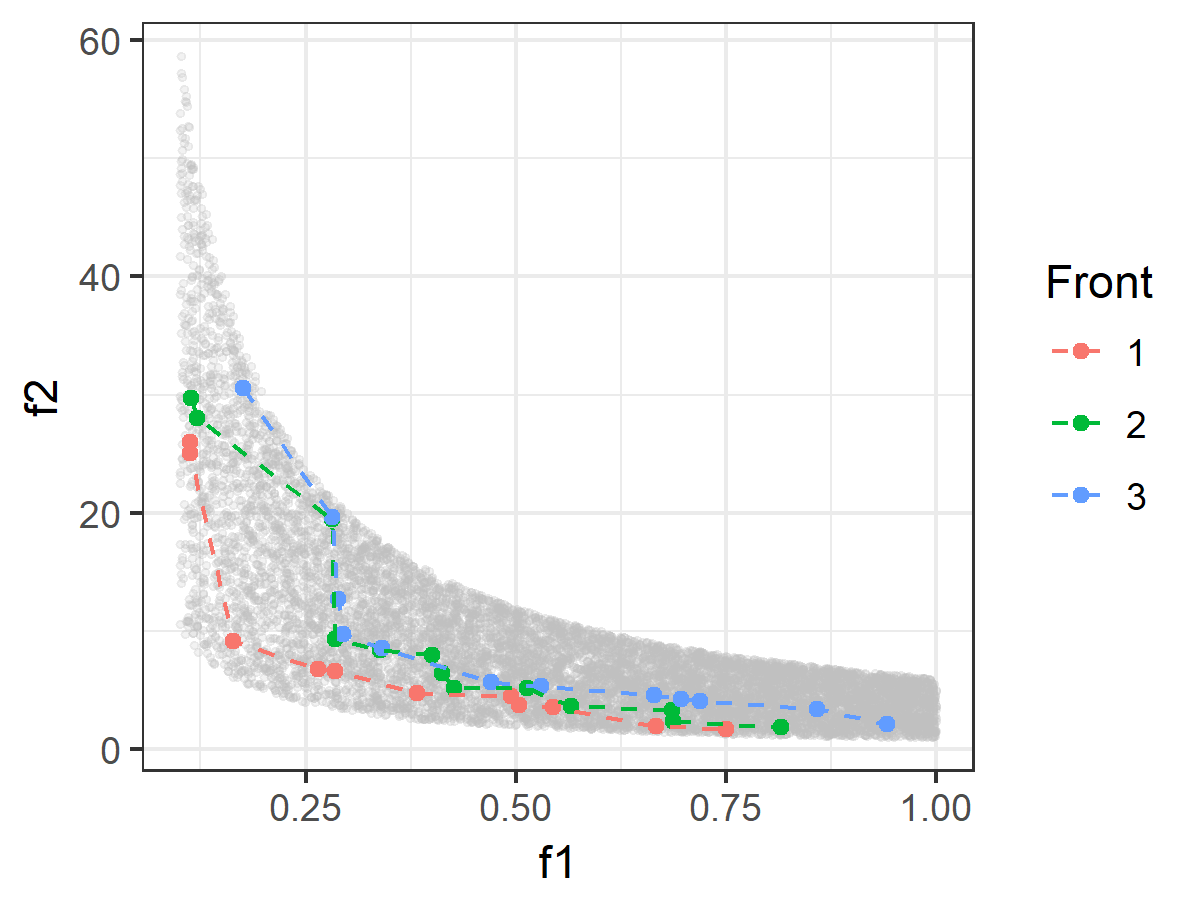
\includegraphics[width = 0.5\linewidth]{figure_man/NSGA2_NDS.png}
\end{center}

\framebreak

How does survival selection now work? We fill $\mu$ \textit{places} one by one with $\mathcal{F}_1, \mathcal{F}_2, ...$ until a front can no longer \textbf{fully} survive (here: $\mathcal{F}_3$).

\begin{center}
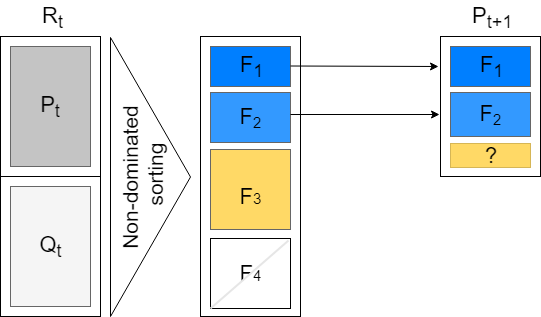
\includegraphics[width = 0.45\linewidth]{figure_man/NSGA2_2.png}
\end{center}

Which individuals survive from $\mathcal{F}_3$? $\to$ \textbf{crowding sort}
\vspace{0.3cm}

\footnotesize{NB: the same principle to rank individuals is applied in tournament selection in parent selection.}
\end{vbframe}



\begin{vbframe}{NSGA-II: crowding distance}
\textbf{Idea:} Add \textit{good} representatives of front $\mathcal{F}_3$, define this as points of $"$low density$"$ in $f$-space.

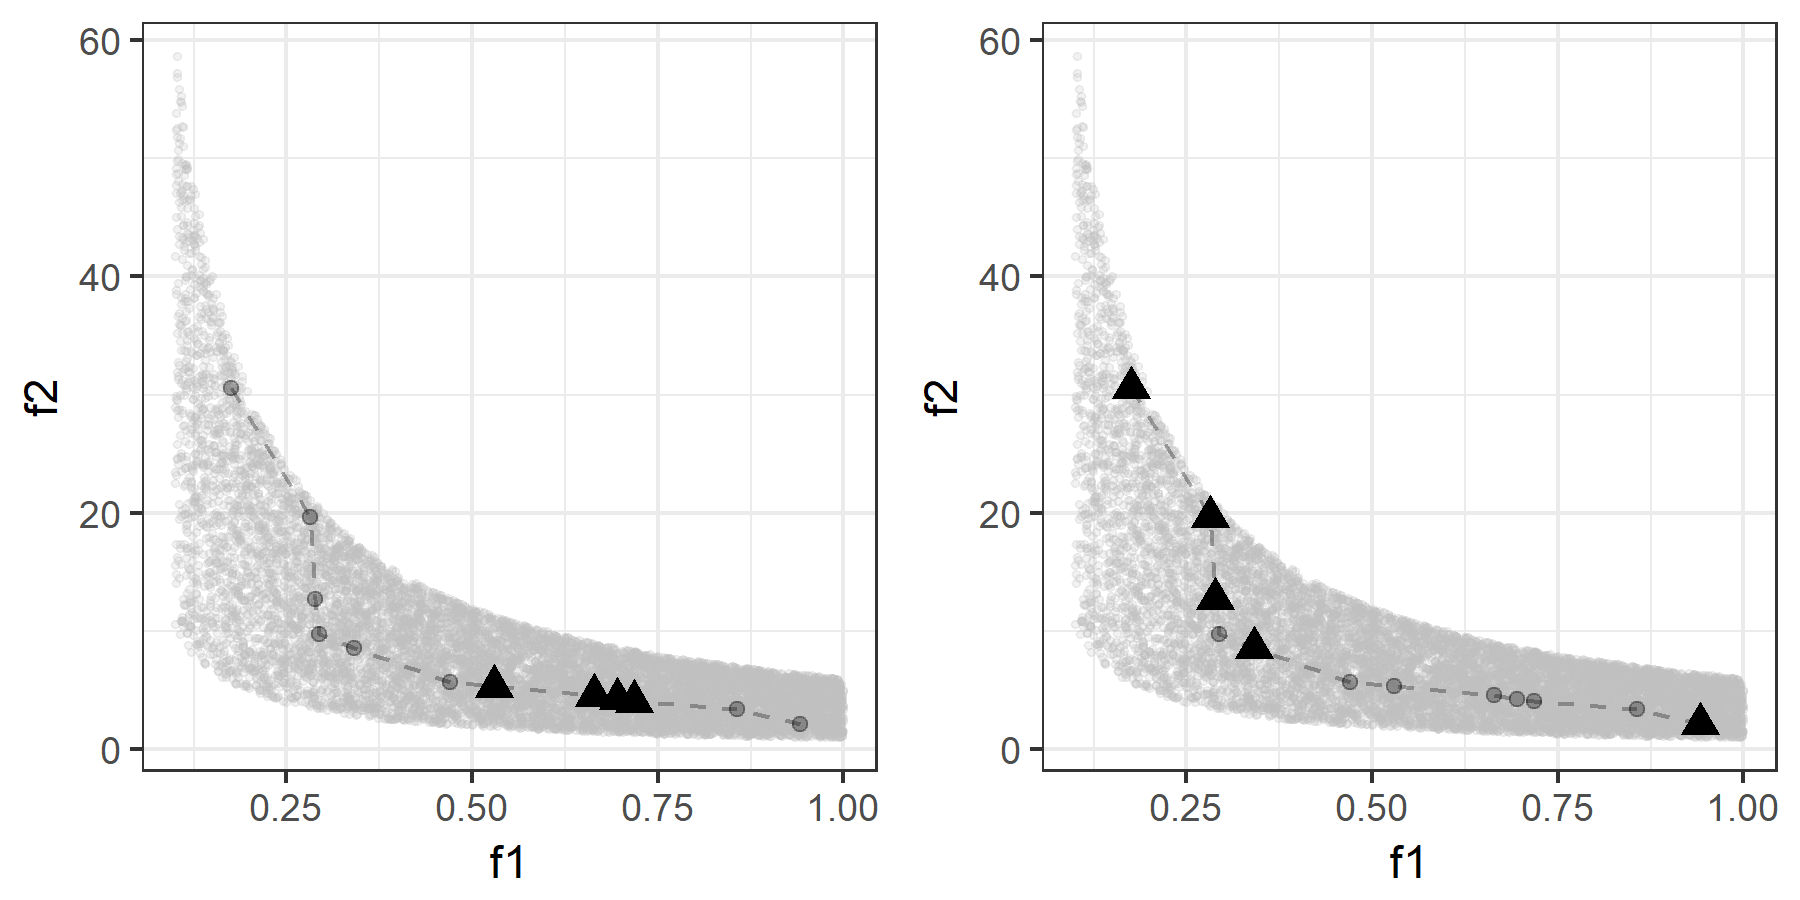
\includegraphics[height = 0.5\textheight]{figure_man/NSGA2_CS1.png}

\begin{footnotesize}
The points on the left (marked by a triangle) do not represent the front very well because they are very close together. The front is better represented by the points on the right plot.
\end{footnotesize}

\framebreak

\begin{columns}
\begin{column}{0.6\textwidth}
\begin{footnotesize}
For each objective $f_j$
\begin{itemize}
\item Sort points by $f_j$
\item Normalize scores to [0,1]
\item Assign border points (which have score 0 or 1) a CD of $\infty$ (they should always be selected, if possible)
\item Each point gets a distance score, which is the distance between its 2 next-neighbors w.r.t. the sorting of $f_j$
\end{itemize}
For each point, all of its $m$ distance scores are summed up (or averaged) and points are ranked w.r.t. to this overall score.
\end{footnotesize}
\end{column}

\begin{column}{0.4\textwidth}
\begin{center}
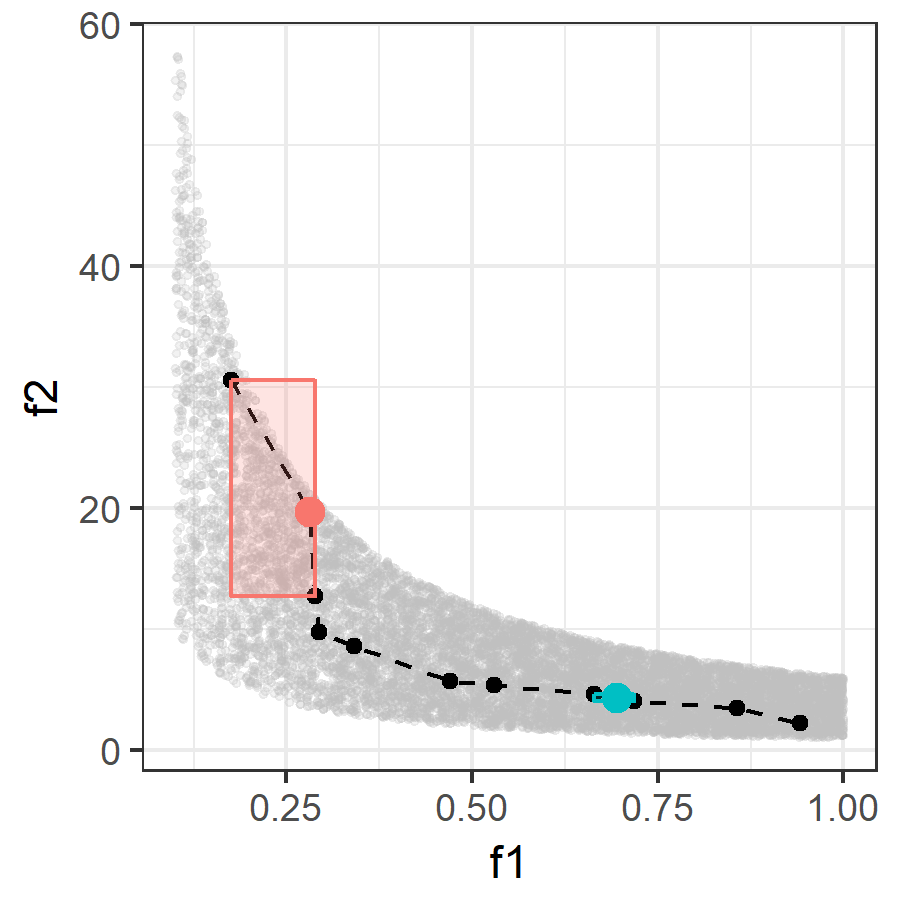
\includegraphics[width = 0.9\linewidth]{figure_man/NSGA2_CS2.png}
\vspace{0.2cm}
\footnotesize{Red: Point with high CD.\\ Blue: Low CD.}
\end{center}
\end{column}
\end{columns}

\end{vbframe}

%\begin{vbframe}
%\begin{algorithm}[H]

 % \begin{center}
  %\caption{NSGA-II}
   % \begin{algorithmic}[1]
   	%\begin{footnotesize}
    %\State Initialize population $P_0$, $t \leftarrow 0$
    %\State $F_1, F_2, F_3, ... \leftarrow \texttt{nondominated-sort}(P_0)$
    %\State Generate $Q_0$ by binary tournament selection, recombination and mutation
     % \Repeat
      %  \State $F_1, F_2, F_3, ... \leftarrow \texttt{nondominated-sort}(P_t \cup Q_t)$
       % \State $i \leftarrow 1$
        %\While{$|P_{t + 1} \cup F_i| < \mu$}
        %	\State $P_{t + 1} = P_{t + 1} \cup F_i$
        %	\State $i \leftarrow i + 1$
    	%\EndWhile
       % \State $\tilde F_i = (\bm{x}_1, \bm{x}_2, ..., \bm{x}_k)= \texttt{SortByCrowdingDistance}(F_i)$
        %\While {$P_{t + 1} < \mu$}
        %	\State $P_{t + 1} = P_{t + 1} \cup \bm{x}_j$
        %	\State $j \leftarrow j + 1$
        %\EndWhile
        %\State Generate $Q_{t + 1}$ by binary tournament selection, recombination and mutation
    %  \Until{Stop criterion fulfilled}
     % \vspace*{-0.3cm}
      %\end{footnotesize}
  %  \end{algorithmic}
   % \end{center}
%\end{algorithm}

%\end{vbframe}




%\textbf{Crowding sort} sorts the individuals based on their crowding distance:

%\begin{itemize}
%\item The crowding distance describes the solution density by one point.
%\item It is calculated from the mean distance to the nearest neighbors around a point in the target function space.
%\item The crowding distance is greater when the neighbors are very far away.
%\item The maximum crowding distance is assigned to the boundary points so that they are always selected.
%\end{itemize}

%\begin{center}
%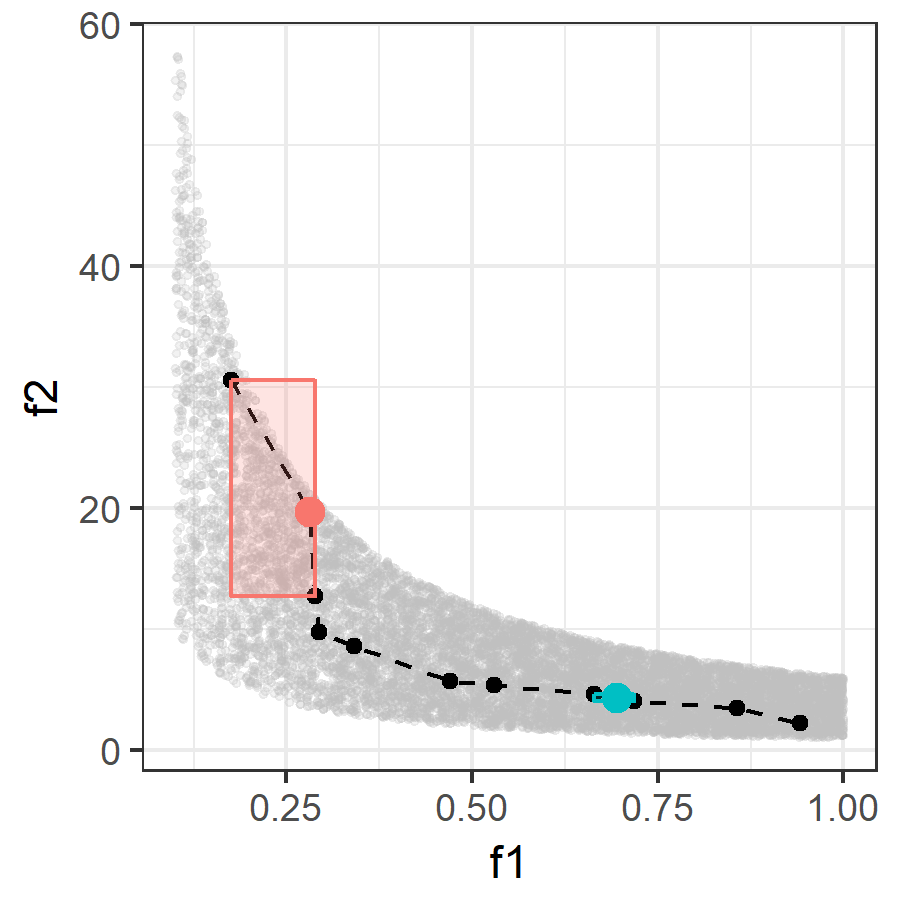
\includegraphics[width = 0.5\linewidth]{figure_man/NSGA2_CS2.png}
%\end{center}

%\begin{footnotesize}
%One point with high crowding distance (red) and one point with very small crowding distance (blue).
%\end{footnotesize}


\begin{vbframe}{Selection criteria: hypervolumen contribiution}
\begin{columns}
\begin{column}{0.6\textwidth}
The SMS-EMOA (S-Metric-Selection-EMOA) evaluates the fitness of an individual $\bm{x} \in \mathcal{P} \subset \Xspace$ based on its contribution to the dominated hypervolume (S-Metric):
$$
\Delta S(\bm{x}, \mathcal{P}) = S(\mathcal{P}, R) - S(\mathcal{P} \setminus \{ \bm{x}\}, R).
$$

\begin{itemize}
\item Dark rectangles: HV contribution of the black dots.
\item Grey point: reference point.
\item The HVC contribution is the volume of space that is dominated only by $\bm{a}$, and nothing else.
\item $\bm{a}^\star$ has lowest S-metric contribution.
\end{itemize}
\end{column}

\begin{column}{0.4\textwidth}
\begin{center}
%Hypervolume contribution in a 2-dimensional objective space:\\
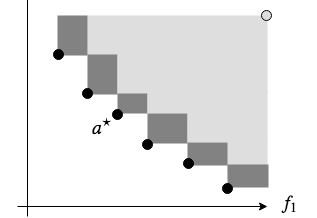
\includegraphics[width = 1\textwidth]{figure_man/hypervolumenbeitrag.png}
\end{center}
\end{column}
\end{columns}

\end{vbframe}


\begin{vbframe}{SMS-EMOA algorithm}

\vspace*{-0.5cm}

\begin{algorithm}[H]
  \begin{center}
  \caption{SMS-EMOA}
    \begin{algorithmic}[1]
    \begin{footnotesize}
    \State Generate start population $P_0$ of size $\mu$
    \State $t \leftarrow 0$
      \Repeat
        \State Generate \textbf{one} individual $\bm{q} \in \R^d$ by recombination and mutation of $P^{[t]}$
        \State $\{\mathcal{F}_{1},..., \mathcal{F}_k\} \leftarrow\text{NDS}(P^{[t]}\cup \{\bm{q}\})$
        \State $\bm{a}^\star \leftarrow \text{argmin}_{\bm{a} \in \mathcal{F}_{k}}\Delta S(\bm{a}, \mathcal{F}_{k})$
        \State $P^{[t+1]} \leftarrow (P^{[t]} \cup \{\bm{q}\}) \setminus\{\bm{a}^\star\}$
        \State $ t \leftarrow t+1$
      \Until{Termination criterion fulfilled}
    \end{footnotesize}
    \vspace*{-0.3cm}
    \end{algorithmic}
    \end{center}
\end{algorithm}

\vspace*{-0.6cm}
\footnotesize
\begin{itemize}
\item L5: the set of temporary $(\mu + 1)$ individuals is partitioned by NDS into $k$ fronts $\mathcal{F}_{1},...,\mathcal{F}_{k}$.
\item L6-7: In last front, find $\bm{a}^\star \in \mathcal{F}_{k}$ with smallest HV contribution - and kill it.
%\item L7: the individual $\bm{a}^\star$ from the worst front with the smallest contribution to the dominated hypervolume does not survive.
\item Fitness of an individual is mainly the rank of its front and HV contribution as tie-breaker.
\end{itemize}
\end{vbframe}

\endlecture
\end{document}


% \begin{vbframe}{SPEA-2}

% Ebenso im Jahr 2002 wurde der \textbf{Strength Pareto EA} (SPEA-2) von Zitzler et al. veröffentlicht.

% \lz

% \begin{itemize}
% \item Neben der aktuellen Population $P_t$ gibt es auch ein sogenanntes Archiv $A_t$, das lediglich zur Bewertung der aktuellen Population dient.

% \begin{figure}
% 	\centering
% 	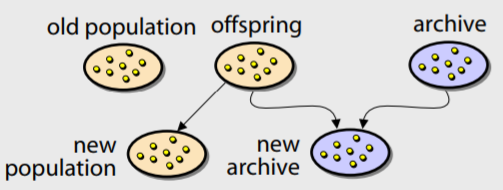
\includegraphics[width=0.6\linewidth]{figure_man/SPEA-archive}
% \end{figure}

% \framebreak

% \item Die Bewertung (und damit auch die Selektion) eines Individuums erfolgt anhand von

% $$
% \text{fitness}(x) = \text{raw}(x) + \text{density}(x).
% $$

% Hierbei ist

% \begin{itemize}
% \item $\text{raw}(x)$ die \enquote{Grundfitness} (bzgl. Population und Archiv)
% \vspace*{-0.2cm}
% $$
% \text{raw}(x) = |\{y \in P_t: f(x) \prec f(y)\}| + |\{y \in A_t: f(x) \prec f(y)\}|,
% $$

% \item $\text{density}(x)$ die Dichte des Punktes
% $$
% \text{density}(x) = \frac{1}{\sigma^{(k)}(x) + 2},
% $$
% ($\sigma^{(k)}$ bezeichne den Abstand zum $k$-nächsten Nachbarn).
% \end{itemize}
% \end{itemize}

% \framebreak

% \begin{algorithm}[H]
% \begin{footnotesize}
%   \begin{center}
%   \caption{SPEA-2}
%     \begin{algorithmic}[1]
%     \State Initialisiere Population $P_0$, $|P_0| = \lambda$ und ein leeres Archiv $A_0, |A_0| = \gamma$
%       \Repeat
%         \State Berechne Fitness der Individuen in $P_t$ und $A_t$ anhand der oben definierten Fitnessfunktion
%         \State Fülle $A_{t+1}$ auf mit nichtdominierten Individuen aus $P_t \cup A_t$ $^{(*)}$
%         \State Fülle \enquote{mating pool} durch binäre Turnierselektion mit Zurücklegen auf $A_{t + 1}$
%         \State Generiere $P_{t + 1}$ durch Rekombination und Mutation
%       \Until{Stoppkriterium erfüllt}
%       \State Gib $A_t$ zurück
%     \end{algorithmic}
%     \end{center}
% \end{footnotesize}
% \end{algorithm}

% \vfill
% \begin{footnotesize}
% $^{(*)}$ Wenn $|A_{t + 1}| > \gamma$, dann entferne solange Individuen mit kleinster Distanz zum Nachbarn, bis $|A_{t + 1}| = \gamma$. Sollte $|A_{t + 1}| < \gamma$, füge die besten dominierten Individuen aus $P_t \cup A_t$ hinzu.
% \end{footnotesize}

% \end{vbframe}



% \textbf{Berechnung des Hypervolumens im 2 dimensionalen Fall:}
% \begin{enumerate}
% \item Sortiere die Zielfunktionsvektoren bzgl. eines Kriteriums (z.B. aufsteigend bzgl. $f_1$)\\
% $\Rightarrow$ Da Pareto-Front (kein Punkt dominiert anderen): Punkte sind bzgl. $f_2$ absteigend sortiert .
% \item Für das $j$-te Individuum $a^{(j)}, j\in \{2,..., |F_{\nu}|\}$ in der sortierten Sequenz der Front $F_{\nu}$ berechnet sich der Hypervolumensbeitrag als:
% \medskip

% $$
% \Delta s(\bm{y}^{(j)}, F_{\nu}) = (y_{1}^{(j+1)} - y_{1}^{(j)}) (y_{2}^{(j-1)} - y_{2}^{(j)})
% $$
% \end{enumerate}




% \item Links: Punkte entsprechen Werten der Individuen in 2-dimensionalem Zielraum.
% \item Links: Punkte ohne Füllung zeigen dominierte Lösungen. Gelbe Fläche zeigt Bereich in dem dominierende Lösungen liegen.


% \begin{vbframe}{SMS-EMOA}
% \textbf{Motivation:}
% \begin{itemize}
% \item Pareto-Front bildet Menge von optimalen Parameterkonbinationen ab.
% \item Oft ist die Menge dieser Kombinationen noch sehr groß.
% \item In Praxis ist es meist nicht möglich alle Pareto-Effizienten Lösungen zu prüfen
% \end{itemize}
% $\Rightarrow$ SMS-EMOA soll möglichst guten Kompromiss zwischen Aufwand der Überprüfung der Paretoeffizienten Lösungen bei gleichzeitig umfassender Abdeckung möglicher Kompromisslösungen darstellen.
% \medskip

% $\Rightarrow$ SMS-EMOA ist einfach handhabbar und verzichtet auf Erstellung eines Archivs um den Aufwand zu reduzieren.
% \medskip

% $\Rightarrow$ Optimierung wird allein auf Grundlage der Population durchgeführt.

% \framebreak
% \end{vbframe}




%
% \item Kombiniert Verfahren von EMOA (NSGA-II als Bewertungskriterium von Lösungen) und Archivierungverfahren (welche Lösungen werden beibehalten?) in einem Algorithmus
% \item NSGA-II wird als Bewertungskriterium für Lösungen herangezogen.
% \item
% \item 


% \end{vbframe}




